\documentclass{book}
\usepackage{commeunjeustyle}
\begin{document}
\chapter*{Dénombrement}
Le dénombrement s'emploie à étudier et à dénombrer divers types de groupements que l'on peut faire à partir d'ensembles finis.
Il est né de l'étude des jeux de hasard et s'est fortement développé sous l'influence du calcul des probabilités, notamment dans une
situation d'équiprobabilité : dans ce cas, en effet, de façon assez intuitive, la probabilité d'un événement
est le rapport entre le nombre d'issues favorables et le nombre total d'issues possibles. Pour cette raison, le dénombrement semble trouver sa place naturelle au début d'un cours de probabilité, même si ses applications sont beaucoup plus diverses dans l'ensemble des mathématiques.\\
La cardinalité est une notion de taille pour les ensembles. Lorsqu'un ensemble est fini, c'est-à-dire si ses éléments peuvent être listés par une suite finie, son cardinal est la longueur de cette suite, autrement dit il s'agit du nombre d'éléments de l'ensemble. En particulier, le cardinal de l'ensemble vide est zéro. Lorsqu'on décompte une collection "sur ses doigts", on crée une bijection entre la collection et ses doigts. On définit naturellement le cardinal comme le nombre de doigts. Il ne s'agit bien entendu pas de revenir au stade du CP et d'apprendre à compter sur ses doigts, mais
bien de définir des objets et notations mathématiques permettant de compter le nombre d'éléments
d'ensembles bien trop gros et compliqués pour être dénombrés à la main.
\section{Cardinal d'un ensemble}
%La clé du dénombrement combinatoire est la notion de bijection : si je peux construire une correspondance
%un-à-un entre les objets d'un ensemble $E$ et les objets d'un ensemble $F$ (c?est-à-dire une bijection de $E$
%dans $F$), alors $E$ a autant d'objets que $F$.
\begin{DefinitionProposition}[Cardinal]
Un ensemble $E$ est \defi{fini} si $E=\emptyset$ ou si il existe $ n\in\N^{\ast}$ tel que $E$ est en bijection avec $\Intf{1}{n}$.\\
Cet entier, $n$, est \impo{unique}, il est appelé le \defi{cardinal} de $E$ noté $\operatorname{Card}{E}$.\\
Si $E=\emptyset$, on pose $\operatorname{Card} E=0$.
\end{DefinitionProposition}
%\ifLEVEL
%\begin{Demonstration}
%Supposons qu'il ne soit pas unique. Par symétrie, il suffit de 
%\end{Demonstration}
%\fi
\begin{Exemple}
Le cardinal des couleurs d'un jeu de carte $\{\clubsuit , \spadesuit, \lozenge,\heartsuit\}$ est 4.  La fonction $f$ définie par \[f(1)=\clubsuit, f(2)=\spadesuit, f(3)=\lozenge, f(4)=\heartsuit\] est bien une bijection entre l'ensemble des couleurs et l'ensemble $\{1,2,3,4\}$.
\end{Exemple}


\begin{Definition}[Dénombrable]
Un ensemble est \defi{dénombrable} s'il est en bijection $\N$.
\end{Definition}
\begin{Exemple}L'ensemble des entiers pairs, noté $2\N$, est dénombrable et infini car la fonction
$$
\Fonction{f}{\N}{2\N}{n}{2n}
$$ 
est bijective.
\end{Exemple}
\begin{Remarque}\label{rq_index}
Les éléments d'un ensemble fini ou dénombrable peuvent être indexés  sous la forme $\{x_i ; i\in I \}$ avec $I=\Intf{1}{n}$ ou $I=\N$ respectivement. Ainsi, on identifie tout ensemble fini de cardinal $n$ à l'ensemble $\Intf{1}{n}$ et tout ensemble dénombrable à $\N$. Par exemple pour les couleurs d'un jeu de carte, on a $\clubsuit \rightarrow 1, \spadesuit \rightarrow 2,  \lozenge \rightarrow 3,  \heartsuit \rightarrow 4 $.   
\end{Remarque}


\begin{Definition}[Équipotent] Deux ensembles (fini ou non) sont \defi{équipotents} ou de \defi{même cardinal} s'il existe une bijection entre eux. 
\end{Definition}



\begin{Exemple}Soient $E=\{1,2,3,4\}$ et $F=\{1,2,3\}$. 
\begin{itemize}
\item Il existe une application surjective de $E$ sur $F$, mais pas d'application injective. 
\item Il existe application injective de $F$ sur $E$, mais pas d'application surjective. 
\end{itemize}
En fait, il n'y a pas assez d'éléments dans $F$ (ou trop peu dans $E$). 
\end{Exemple} 


\section{Principes fondamentaux de dénombrement}

\begin{Methode}[Modélisation avec une urne]\normalfont Un problème d'urne est une représentation d'expériences aléatoires par un tirage aléatoire uniforme de boules dans une urne. L'urne est supposée contenir un  nombre de boules numérotés de $1$ à $n$,\setlength{\unitlength}{1mm}
 qui sont indiscernables au toucher, c'est-à-dire que lorsque l'on tire une boule à l'intérieur, le tirage est aléatoire et chaque boule à l'intérieur de l'urne a la même chance d'être tirée. 
\begin{center}
 \begin{picture}(25,25)
\put(0,5){
\put(0,0){\line(0,1){20}}
\put(0,0){\line(1,0){20}}
\put(20,0){\line(0,1){20}}

\put(15,13){\circle{5}}
\put(14,12){\text{$1$}}

\put(9,11){\circle{5}}
\put(8,10){\text{$3$}}

\put(16,3){\circle{5}}
\put(15,2){\text{$4$}}

\put(5,5){\circle{5}}
\put(4,4){\text{$2$}}}
\put(0,0){Urne de 4 boules}
\end{picture}
\end{center}
Il y a deux critères pour distinguer ces tirages au sort :
\begin{itemize}
\item l'\defi{ordre} dans lequel on tire les boules est pris en considération, on dit que
c'est un « tirage avec ordre », sinon on parle d'un « tirage sans ordre ». Avec ordre, le tirage est noté avec des parenthèses pour un $p$-uplet \footnote{Un $p$-uplet  est une collection ordonnée de $p$ éléments d'un même ensemble, par exemple, le $2$-uplet $(x_1,x_2)\in \R^2$ est un vecteur du plan.}
et sans ordre, avec des accolades pour un ensemble
% (l'ensemble des boules du tirage est une partie de l'ensemble des boules de l'urne\footnote{Un ensemble E est une collection d'éléments dont l'ordre n'a pas d'importance
%(ainsi, les ensembles $\{2, 3\}$ et $\{3, 2\}$ sont les mêmes ensembles) et comptés sans multiplicité
%(par exemple, $\{2,2\}=\{2\}$). On note $x \in A$ si x appartient à l'ensemble $A$. Si $A$ et $B$ sont deux
%ensemble, on écrit $A \subset B$ et on dit que $A$ est inclus dans $B$ si chaque élément de $A$ appartient à
%$B$. L'ensemble vide, qui ne contient aucun élément, est noté $\emptyset$}).
Par exemple, pour le tirage des boules 7, 33 et 24, avec ordre, on note $(7,33,24)$ et sans ordre $\{7,33,24\}$. Remarque, on a bien entendu $\{7,33,24\}=\{33,24,7\}$ par contre $(7,33,24)\neq (33,24,7)$.
\item la \defi{répétition} si on remet chaque boule tirée dans l'urne avant de tirer la suivante, on peut
tirer plusieurs fois la même boule : on parle alors d'un tirage \defi{avec remise} et dans la cas contraire on parle d'un tirage
\defi{sans remise}.
\end{itemize}
\end{Methode}
\begin{Exemple} La question : « Dans une course de chevaux avec 10 participants, de combien de
façons peut-on parier pour le tierce ? » peut être reformulée de la manière
suivante : « De combien de façons peut-on tirer avec ordre et sans remise 3 boules d'une urne qui en
contient 10 ? ».
\end{Exemple}
\begin{Methode}[Décomposition]\normalfont Si une opération globale peut se décomposer en $k$ opérations élémentaires successives,
ces dernières pouvant s'effectuer respectivement de $n_1, n_2, ..., n_k$ manières, alors
l'opération globale peut se faire de $n_1 n_2 ... n_k$ manières différentes.
\end{Methode}
\begin{Exemple}Les localités X et Y sont reliées par trois routes a, b et c et les localités Y et Z par deux
routes d et e. Combien y a-t-il de trajets de X à Z en passant par Y ?\\
\begin{center}
\includegraphics[width=5cm]{chemin.png}
\end{center}
Il y a 6= 3·2 trajets possibles : (a, d), (a, e), (b, d), (b, e), (c, d) et (c, e).
\end{Exemple}
\begin{Methode}[Double-comptage] \normalfont Il consiste à établir une égalité en comptant de deux manières différentes une certaines quantité. 
\end{Methode}
\begin{Exemple}
Un berger ne voyant que les pattes de ses moutons pourra déterminer le nombre d'animaux en divisant le nombre de pattes par quatre. Le berger a compté le nombre de pattes de deux manières différentes : l'un directement, l'autre avec le principe de décomposition.  
\end{Exemple}
\section{Tirage avec ordre et avec remise}
\begin{Proposition} Le nombre de tirages différents avec remise et avec ordre dans une urne $n$ boules en tirant $p$ boules est  $n^p$.
\end{Proposition}

\begin{Demonstration} 
Il y a $n$ façons de tirer la première boule, puis $n$ façons de tirer la seconde boule et ainsi de suite, d'où, après le principe de décomposition, en totalité $\overbrace{n.n.\dots.n}^{p \text{ fois}}=n^p$ façons.
\begin{center}
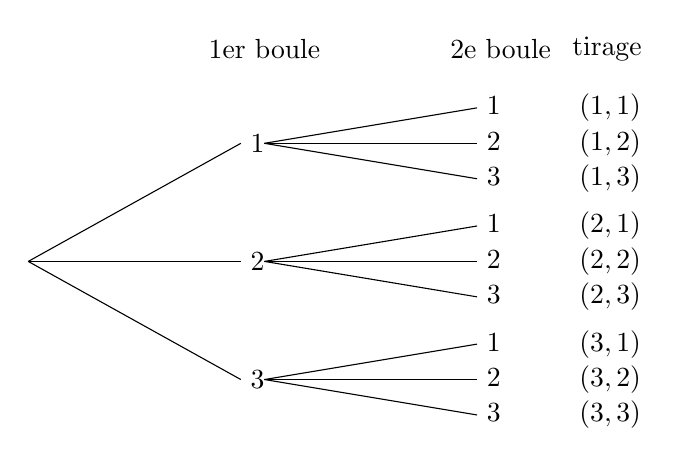
\begin{tikzpicture}[scale=1.5]
\node at (2,1.8) {1er boule };
\node at (4,1.8) {2e boule};
\node at (4.9,1.8) {tirage};
\draw  (0,0)  -- (1.8,1) node[right]{$1$};
\draw  (2,1)  -- (3.8,1.3) node[right]{$1 \hspace{1cm} (1,1)$};
\draw  (2,1)  -- (3.8,1) node[right]{$2   \hspace{1cm} (1,2)$};
\draw  (2,1)  -- (3.8,0.7) node[right]{$3  \hspace{1cm}  (1,3)$};
\draw  (0,0)  -- (1.8,0) node[right]{$2$};
\draw  (2,0)  -- (3.8,0.3) node[right]{$1 \hspace{1cm}   (2,1)$};
\draw  (2,0)  -- (3.8,0) node[right]{$2  \hspace{1cm}  (2,2)$};
\draw  (2,0)  -- (3.8,-0.3) node[right]{$3  \hspace{1cm}  (2,3)$};
\draw  (0,0)  -- (1.8,-1) node[right]{$3$};
\draw  (2,-1)  -- (3.8,-0.7) node[right]{$1 \hspace{1cm}   (3,1)$};
\draw  (2,-1)  -- (3.8,-1) node[right]{$2  \hspace{1cm}  (3,2)$};
\draw  (2,-1)  -- (3.8,-1.3) node[right]{$3  \hspace{1cm}  (3,3)$};
\end{tikzpicture}\\
Diagramme en arbre d'un tirage avec ordre et avec remise  dans une urne de 3 boules en tirant 2 boules.
\end{center}

\end{Demonstration}


\begin{Corollaire}[Cardinal d'un produit cartésien]Soit $E$  de cardinal $n$.\\ Alors $card(E^p)=n^p$.
\end{Corollaire}


\begin{Demonstration} Soit un p-uplet $(x_1,\dots,x_p)\in E^p$. Pour chaque coordonnée $x_i$, $i$ représente le numéro du tirage et $x_i$ le numéro de la boule. $(x_1,\dots,x_p)$ représente un tirage avec ordre et avec remise dans une urne $n$ boules en tirant $p$ fois. 
En conclusion le cardinal $E^p$ est le nombre  de tirages différents avec remise et avec ordre dans une urne $n$ boules en tirant $p$ boules, soit  $n^p$.
\end{Demonstration}
\begin{DefinitionProposition}[p-uplet] Soit $E$  de cardinal $n$ et $p\in\N^*$.\\
On appelle \defi{p-liste} de $E$ ou \defi{p-uplet} de $E$ tout élément de $E^p$. Un 2-uplet est un \defi{couple}.  Un 3-uplet est un \defi{triplet}.\\ 
Il existe $n^p$ p-uplet de $E$.
\end{DefinitionProposition}
\begin{Exemple} Combien de combinaisons à quatre chiffres peut-on former avec les chiffres de 0 à 9 ?\\
Une combinaison est un 4-uplet de $\Intf{0}{9}$ correspondant à un tirage avec ordre et avec remise  dans une urne de 10 boules en tirant 4 fois.   Donc le nombre de combinaisons est $10^4$.
\end{Exemple}
\begin{Corollaire}[Nombre d'applications entre deux ensembles]\label{diff}Soit $E$  de cardinal $p$ et $F$ de cardinal $n$.\\ Alors le cardinal de l'ensemble 
des applications de $E$ dans $F$ est égale à  $n^p$.
\end{Corollaire}
\begin{Demonstration} D'après la remarque~\ref{rq_index}, l'ensemble $E$  de cardinal $p$ est identifié à $\Intf{1}{p}$ et l'ensemble $F$ de cardinal $n$ à $\Intf{1}{n}$.  La fonction $\phi$ définie par :
\[
\Fonction{\phi}{\left\{ f\in\Intf{1}{p}\to \Intf{1}{n}\right\} }{ \Intf{1}{n}^p}{f}{\left (f(1),f(2),\dots, f(p)\right )}
\]
associe à chaque  numéro du tirage, $i$, le numéro de  de la boule $f(i)$. Elle est bijective.\\
Comme l'ensemble d'arrivée de la fonction $\phi$ est l'ensemble des tirages avec remise et avec ordre, de cardinal $n^p$, le cardinal de l'ensemble des applications $E$ dans $F$ est bien $n^p$.
\end{Demonstration}


\section{Tirage avec ordre et sans remise}
\begin{Definition}[Factoriel] Le nombre $\prod_{i=1}^ni= 1\times 2\times \dots  times (n-1)\times n$ est appelé \defi{factorielle} $n$ et
est noté $n!$.
\end{Definition}
\begin{DefinitionProposition}[Arrangement]\label{proparran}
Un tirage sans remise et avec ordre dans une urne $n$ boules en tirant $p$ boules correspond à p-uplet d'éléments distincts.\\
Le nombre de tirages différents  avec $p\leq n$  est $\frac{n!}{(n-p)!}$.\\
 On l'appelle \defi{arrangement}  et on le note $A^p_n$.
\end{DefinitionProposition}
\begin{Demonstration} Comme on a $n$ façons de tirer la première boule, puis $n-1$ façons de tirer la seconde boule et ainsi de suite, d'après le principe de décomposition, on obtient $n.(n-1)\dots(n-p+1)=\frac{n.(n-1)\dots(n-p+1).(n-p).(n-p-1)\dots 2.1}{(n-p).(n-p-1)\dots 2.1}=\frac{n!}{(n-p)!}$.
\begin{center}
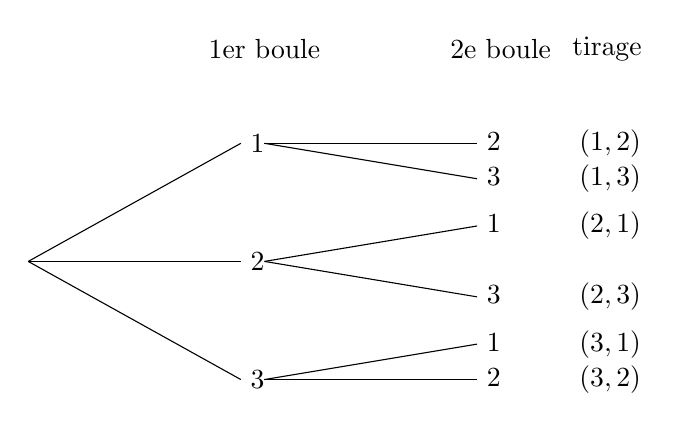
\begin{tikzpicture}[scale=1.5]
\node at (2,1.8) {1er boule };
\node at (4,1.8) {2e boule};
\node at (4.9,1.8) {tirage};
\draw  (0,0)  -- (1.8,1) node[right]{$1$};
\draw  (2,1)  -- (3.8,1) node[right]{$2   \hspace{1cm} (1,2)$};
\draw  (2,1)  -- (3.8,0.7) node[right]{$3  \hspace{1cm}  (1,3)$};
\draw  (0,0)  -- (1.8,0) node[right]{$2$};
\draw  (2,0)  -- (3.8,0.3) node[right]{$1 \hspace{1cm}   (2,1)$};
\draw  (2,0)  -- (3.8,-0.3) node[right]{$3  \hspace{1cm}  (2,3)$};
\draw  (0,0)  -- (1.8,-1) node[right]{$3$};
\draw  (2,-1)  -- (3.8,-0.7) node[right]{$1 \hspace{1cm}   (3,1)$};
\draw  (2,-1)  -- (3.8,-1) node[right]{$2  \hspace{1cm}  (3,2)$};
\end{tikzpicture}\\
Diagramme en arbre d'un tirage avec ordre et avec remise  dans une urne de 2 boules en tirant 2 fois.
\end{center}
\end{Demonstration}



\begin{Exemple} Dans une course de chevaux avec 10 participants, de combien de
façons peut-on parier pour le tierce ? \\
Un tierce correspond à un tirage avec ordre et sans remise dan une urne de 10 boules en tirant 3 boules. Donc le nombre de tierce est $A^3_{10}=8.9.10=720$
\end{Exemple}
\begin{Corollaire}[Nombre d'applications injectives entre deux ensembles]
Soit $E$ de cardinal $p$ et $F$ de cardinal $n$ avec  $n$ et $p$ deux entiers non nuls. \\
Alors le cardinal de l'ensemble des applications injectives de $E$ dans $F$  est égale à  $A^p_n$.
\end{Corollaire}
\begin{Demonstration}Idem que la démonstration du corolaire~\ref{diff} sauf que, comme le tirage est sans remise, les numéros de chaque boule sont différents deux à deux. Cela implique l'injectivité de la fonction.
\end{Demonstration}
\begin{Corollaire}[$n=p$]Le nombre de tirages différents sans remise et avec ordre dans une urne $n$ boules en tirant toutes les boules est $n!$.
\end{Corollaire}
\begin{Exemple}Pour 3 boules, on a $6=3.2.1$ manières \includegraphics[scale=0.1]{permutation_bille.png}
\end{Exemple}
\begin{DefinitionProposition}[Permutation (cas n=p)]
Tout classement ordonné de $n$ éléments distincts correspondant à un triage avec ordre de toutes les boules est une \defi{permutation} de ces $n$
éléments. \\
Lorsque l'ensemble $E = \Intf{1}{n}$, on note \defi{$S_n$} l'ensemble des permutations, soit l'ensemble des bijections de $E$ sur lui même. Cet ensemble possède une structure de groupe, on l'appelle \defi{groupe symétrique}.\\
On a $\operatorname{Card}(S_n)=n!$.
\end{DefinitionProposition}
\begin{Exemple} Par exemple la liste $(1,3,2,5,4)$ est la permutation $\sigma$ telle que $\sigma(1)=1, \sigma(2)=3, \sigma(3)=2, \sigma(4)=5 \text{ et }\sigma(5)=4$ que l'on peut écrire   
$\sigma =\begin{pmatrix}
1 & 2 & 3 & 4 & 5 \\
1 & 3 & 2 & 5 & 4
\end{pmatrix}$.
\end{Exemple} 
\section{Tirage sans ordre et sans remise}
\begin{center}
\includegraphics[width=0.5\textwidth]{bd_combinatoire.png}
\end{center}

\begin{DefinitionProposition}[Combinaison]\label{propcomb} 
Un tirage sans remise et sans ordre dans une urne $n$ boules en tirant $p$ boules avec $p\leq n$  est appelé \defi{combinaison}. Le nombre de combinaisons est égale au  coefficient binomial, $\begin{pmatrix}n\\p\end{pmatrix}$, tel que $$\begin{pmatrix}n\\p\end{pmatrix}=\frac{n!}{p!(n-p)!}.$$ 
Pour $p>n$, on pose $\begin{pmatrix}n\\p\end{pmatrix}=0$ 
\end{DefinitionProposition}
\begin{Demonstration}Avec le principe de double-comptage, on dénombre le nombre d'arrangements de deux façons différentes. L'un d'après la proposition~\ref{proparran}, on a $A_p^n=\frac{n!}{(n-p)!}$, et l'autre on commence par choisir une combinaison de $p$ boules parmi $n$ ($\begin{pmatrix}n\\p\end{pmatrix}$ configurations possibles
de choisir) et on l'ordonne par permutation des boules pour obtenir tous les
arrangements simples ($p!$ configurations possibles
de les ordonner), soit d'après le principe de décomposition $p!\begin{pmatrix}n\\p\end{pmatrix}$. D'où $p!\begin{pmatrix}n\\p\end{pmatrix}=\frac{n!}{(n-p)!}$, donc $\begin{pmatrix}n\\p\end{pmatrix}=\frac{n!}{p!(n-p)!}$.
\end{Demonstration}
\begin{Exemple} Le nombre de tirages au Loto (5 numéros parmi 49) est  $\begin{pmatrix}49\\5\end{pmatrix}=1 906 884$.
\end{Exemple}
\begin{Exemple} Le nombre d'anagrammes $00111$ est $\begin{pmatrix}5\\3\end{pmatrix}$. Un anagramme est une combinaison où les positions des 1 dans le mot correspond au résultat d'un tirage sans remise et sans ordre dans une urne numérotée de  $5$ boules en tirant $3$ boules. Par exemple, l'anagramme  $01101$ correspond au tirage $\{2,3,5\}$.
\end{Exemple}
\begin{Corollaire}[Nombre de parties $p$ éléments d'un ensemble]
Le nombre de configurations de sous-ensemble à $p$ éléments d'un ensemble à $n$ éléments est $\begin{pmatrix}n\\p\end{pmatrix}$.
\end{Corollaire}
\begin{Demonstration}Soit $E=\Intf{1}{n}$. Soit $A=\{i_1,i_2,\dots,i_p\}$ un sous-ensemble de p éléments de $E$. L'ensemble $A$ correspond bien à un tirage sans ordre et sans remise dans une urne $n$ boules en tirant $p$ boules. CQFD. 
\end{Demonstration}




\begin{Proposition}
\begin{enumerate}
\item $\forall n \in \N, \begin{pmatrix}n\\0\end{pmatrix}=\begin{pmatrix}n\\n\end{pmatrix}=1$
\item $\forall n \in \N, \begin{pmatrix}n\\1\end{pmatrix}=\begin{pmatrix}n\\n-1\end{pmatrix}=n$
\item $\forall n,p \in \N,\text{ avec }p\leq n \begin{pmatrix}n\\p\end{pmatrix}=\begin{pmatrix}n\\n-p\end{pmatrix}$
\item Formule de Pascale : $\forall n,p \in \N,\text{ avec }p\leq n, \quad \begin{pmatrix}n-1\\p-1\end{pmatrix}+\begin{pmatrix}n-1\\p\end{pmatrix}=\begin{pmatrix}n\\p\end{pmatrix}$
\end{enumerate}
\end{Proposition}
\begin{Demonstration}
Argumentation combinatoire :
\begin{enumerate}
\item une urne à $n$ boules a un unique tirage à zéro boule, l'ensemble vide $\emptyset$, et un unique tirage de n boule, lui-même
\item une urne de $n$ boules a $n$ tirages à une boule pour la première boule
\item choisir $p$ boules parmi $n$ revient à sélectionner les $n - k$ boules qu'on ne choisira pas.
\item Dénombrons par principe de double-comptage l'ensemble des combinaisons de $p$ boules parmi $n$. D'abord, la proposition~\ref{propcomb} nous donne $\begin{pmatrix}n\\p\end{pmatrix}$.\\
Puis on recherche le nombre d'anagrammes comportant $p$ 0 et $(n-p)$ 1. On sépare en deux cas sur la dernière lettre du mot :
\begin{itemize}
\item \textit{égale à 0} : les anagrammes de la forme $\overbrace{*\dots*}^{n-1 \text{ lettres}}0$ doivent comporter $p-1$ zéro parmi $n-1$ lettres pour être un anagramme de  $p$ zéro parmi $n$ lettres. Son cardinal est   $\begin{pmatrix}n-1\\p-1\end{pmatrix}$,
\item \textit{égale à 1} : les anagrammes de la forme $\overbrace{*\dots*}^{n-1 \text{ lettres}}1$ doivent comporter $p$ zéro parmi $n-1$ lettres pour être un anagramme de  $p$ zéro parmi $n$ lettres. Son cardinal est   $\begin{pmatrix}n-1\\p\end{pmatrix}$,
\end{itemize}   
Au total on a donc $\begin{pmatrix}n-1\\p-1\end{pmatrix}+\begin{pmatrix}n-1\\p\end{pmatrix}$ d'anagrammes, soit le nombre 
de combinaisons de $p$ boules parmi $n$ d'où le résultat.\\
%Dis autrement, on sépare en deux cas : ceux contenant la boule $n$ qui sont l'ensemble des combinaison de $p-1$ boules parmi $n-1$  au nombre $\begin{pmatrix}n-1\\p-1\end{pmatrix}$ et ceux ne contenant pas la boule $n$  qui sont l'ensemble des combinaison de $p$ boules parmi $n-1$  au nombre $\begin{pmatrix}n-1\\p\end{pmatrix}$. Au total on a donc $\begin{pmatrix}n-1\\p-1\end{pmatrix}+\begin{pmatrix}n-1\\p\end{pmatrix}$
%des combinaison de $p$ boules parmi $n$ d'où le résultat.
\end{enumerate}
La formule de Pascal nous permet de construire le triangle de Pascal.
\begin{center}
\begin{tabular}{c|ccccccc}
\multicolumn{1}{l}{$n$} &&&&&&&\\\cline{1-1} 
0 &1&&&&&&\\
1 &1&1&&&&&\\
2 &1&2&1&&&&\\
3 &1&3&3&1&&&\\
4 &1&4&6&4&1&&\\
5 &1&5&10&10&5&1&\\
6 &1&6&15&20&15&6&1\\\hline
\multicolumn{1}{l}{} &0&1&2&3&4&5&6\\\cline{2-8}
\multicolumn{1}{l}{} &\multicolumn{7}{c}{$p$}
\end{tabular}
\end{center}
\end{Demonstration}


\begin{Proposition}[Formule du binôme de Newton] Soit $x, y$ des nombres réels et $n > 1$ un
entier. \\
Alors :
\[
(x+y)^n= \sum_{p=0}^n \begin{pmatrix}n\\p\end{pmatrix} x^p y^{n-p}
\]
\end{Proposition}
\begin{Demonstration} Lorsqu'on développe $(x+y).(x+y) \dots (x+y)$, pour trouver le coefficient
devant $x^p y^{n-p}$, parmi les $n$ facteurs $(x + y)$, il faut en choisir $p$ pour lesquels on garde le $x$ et
qui vont donner un terme $x^p$, et les $n - p$ autres facteurs pour lesquels on sélectionne $y$ (et qui
sont fixés par le choix des $p$ premiers) vont donner le terme $y^{n-p}$. Le résultat s'ensuit.
\end{Demonstration}



\impo{Synthèse} :

Tirage de $p$ boules dans une urne en contenant $n$.\\
\begin{tabular}{c|c|c}
 & avec remise  & sans remise\\ \hline
 avec ordre &  $n^p$ &  $A^p_n=\frac{n!}{(n-p)!}$, si $n=p$ $A_n^p=n!$\\  \hline
 sans ordre &        & $\begin{pmatrix}n\\p\end{pmatrix} =\frac{n!}{p!(n-p)!}$
\end{tabular}
\end{document}
